%
% Szakdolgozatminta az Eszterházy Károly Katolikus Egyetem
% matematika illetve informatika szakos hallgatóinak.
%

\documentclass[
% opciók nélkül: egyoldalas nyomtatás, elektronikus verzió
% twoside,     % kétoldalas nyomtatás
% tocnopagenum,% oldalszámozás a tartalomjegyzék után kezdődik
]{thesis-ekf}
\usepackage[T1]{fontenc}
\PassOptionsToPackage{defaults=hu-min}{magyar.ldf}
\usepackage[magyar]{babel}


%\usepackage{listingsutf8,mathtools,amssymb,amsthm,pdfpages,xurl}
\usepackage{listingsutf8,lmodern,caption,mathtools,amssymb,amsthm,pdfpages,xurl,float}

\footnotestyle{rule=fourth}

\newtheorem{tetel}{Tétel}[chapter]
\theoremstyle{definition}
\newtheorem{definicio}[tetel]{Definíció}
\theoremstyle{remark}
\newtheorem{megjegyzes}[tetel]{Megjegyzés}

\makeatletter
\expandafter\let\csname active@char\string?\endcsname\relax
\expandafter\let\csname active@char\string!\endcsname\relax
\expandafter\let\csname active@char\string:\endcsname\relax


\initiate@active@char{?}
\initiate@active@char{!}
\initiate@active@char{:}
\makeatother

\lstset{
    language=[Sharp]C,
    inputencoding=utf8/latin2,
    basicstyle=\footnotesize\ttfamily,
    columns=fullflexible,
    numbers=left,
    breaklines,
    xleftmargin=0.7cm,
    xrightmargin=0.7cm,
    frame=ltrb,
    rulecolor=\color{blue!80!black},
    backgroundcolor=\color{gray!30},
    commentstyle=\color{green!60!black},
    keywordstyle=\color{blue},
    morekeywords={using,public,class,int,void,new,for,bool,false,true,if},
}
\renewcommand{\lstlistingname}{kód}



\begin{document}

\institute{Matematikai és Informatikai Intézet}
\title{Mesterséges intelligencia a számítógépes játékokban}
\author{Pataki Tamás\\Programtervező Informatikus BSc}
\supervisor{Dr. Kovásznai Gergely\\Egyetemi docens}
\city{Eger}
\date{2025}
\maketitle

\tableofcontents

\chapter*{Bevezetés}
\addcontentsline{toc}{chapter}{Bevezetés}

A szakdolgozati téma választás idején sok lehetőség volt elérhető számomra. Végül amikor választanom kellet olyan témát szerettem volna amely egy sajátos kihívást ad és egyben az érdekeltségi közömbe is tartozik. A számítógépes játékok és azoknak a fejlesztése már korábban is érdekelt, és ez adta meg a löketet a téma választásához.

A témám egy olyan játék készítése, mely

Emellett a harckocsik között történő csaták is érdekelnek, főleg a II. világháborúban használatos fegyverekkel. Emiatt egy olyan játékot szerettem volna fejleszteni melyben meglehetett tapasztalni az akkori időben kifejlesztetett harckocsiknak az erejét. Csavarként gondoltam ki azt a funkciót, hogy a különböző harckocsik elemeit meglehessen cserélni egymás közt, ezzel új lehetőségeket nyitva a taktikákra és egy fantázia elemet belerakva a játékba.

Emiatt választottam a projektem megvalósítására Unity\cite{unity} játékmotort, mely lehetőséget adott ennek kifejlesztésére 3D térben.



A szakdolgozatom az alábbi linken érhető el: \url{https://github.com/patakitamas2002/Tank-Game}

\chapter{Tématerület áttekintése}

\section{Inspiráció}

Inspirációmat főként a War Thunder\cite{warthunder} című játékból merítettem, mely egy több mint 10 éve kiadott, de folyamatosan tovább fejlesztett, online többszereplős játék. Többféle járművet lehet benne irányítani, például repülők, hajók, helikopterek, de főleg a harckocsis részéből merítettem az ötleteimet. Több ezer jármú elérhető benne és mélyen kidolgozott rendszereik vannak, melyek a realizmusra törekednek. Ennek egy töredékét szerettem volna elérni egy félig realisztikus megoldással.


\begin{figure}[H]
    \centering
    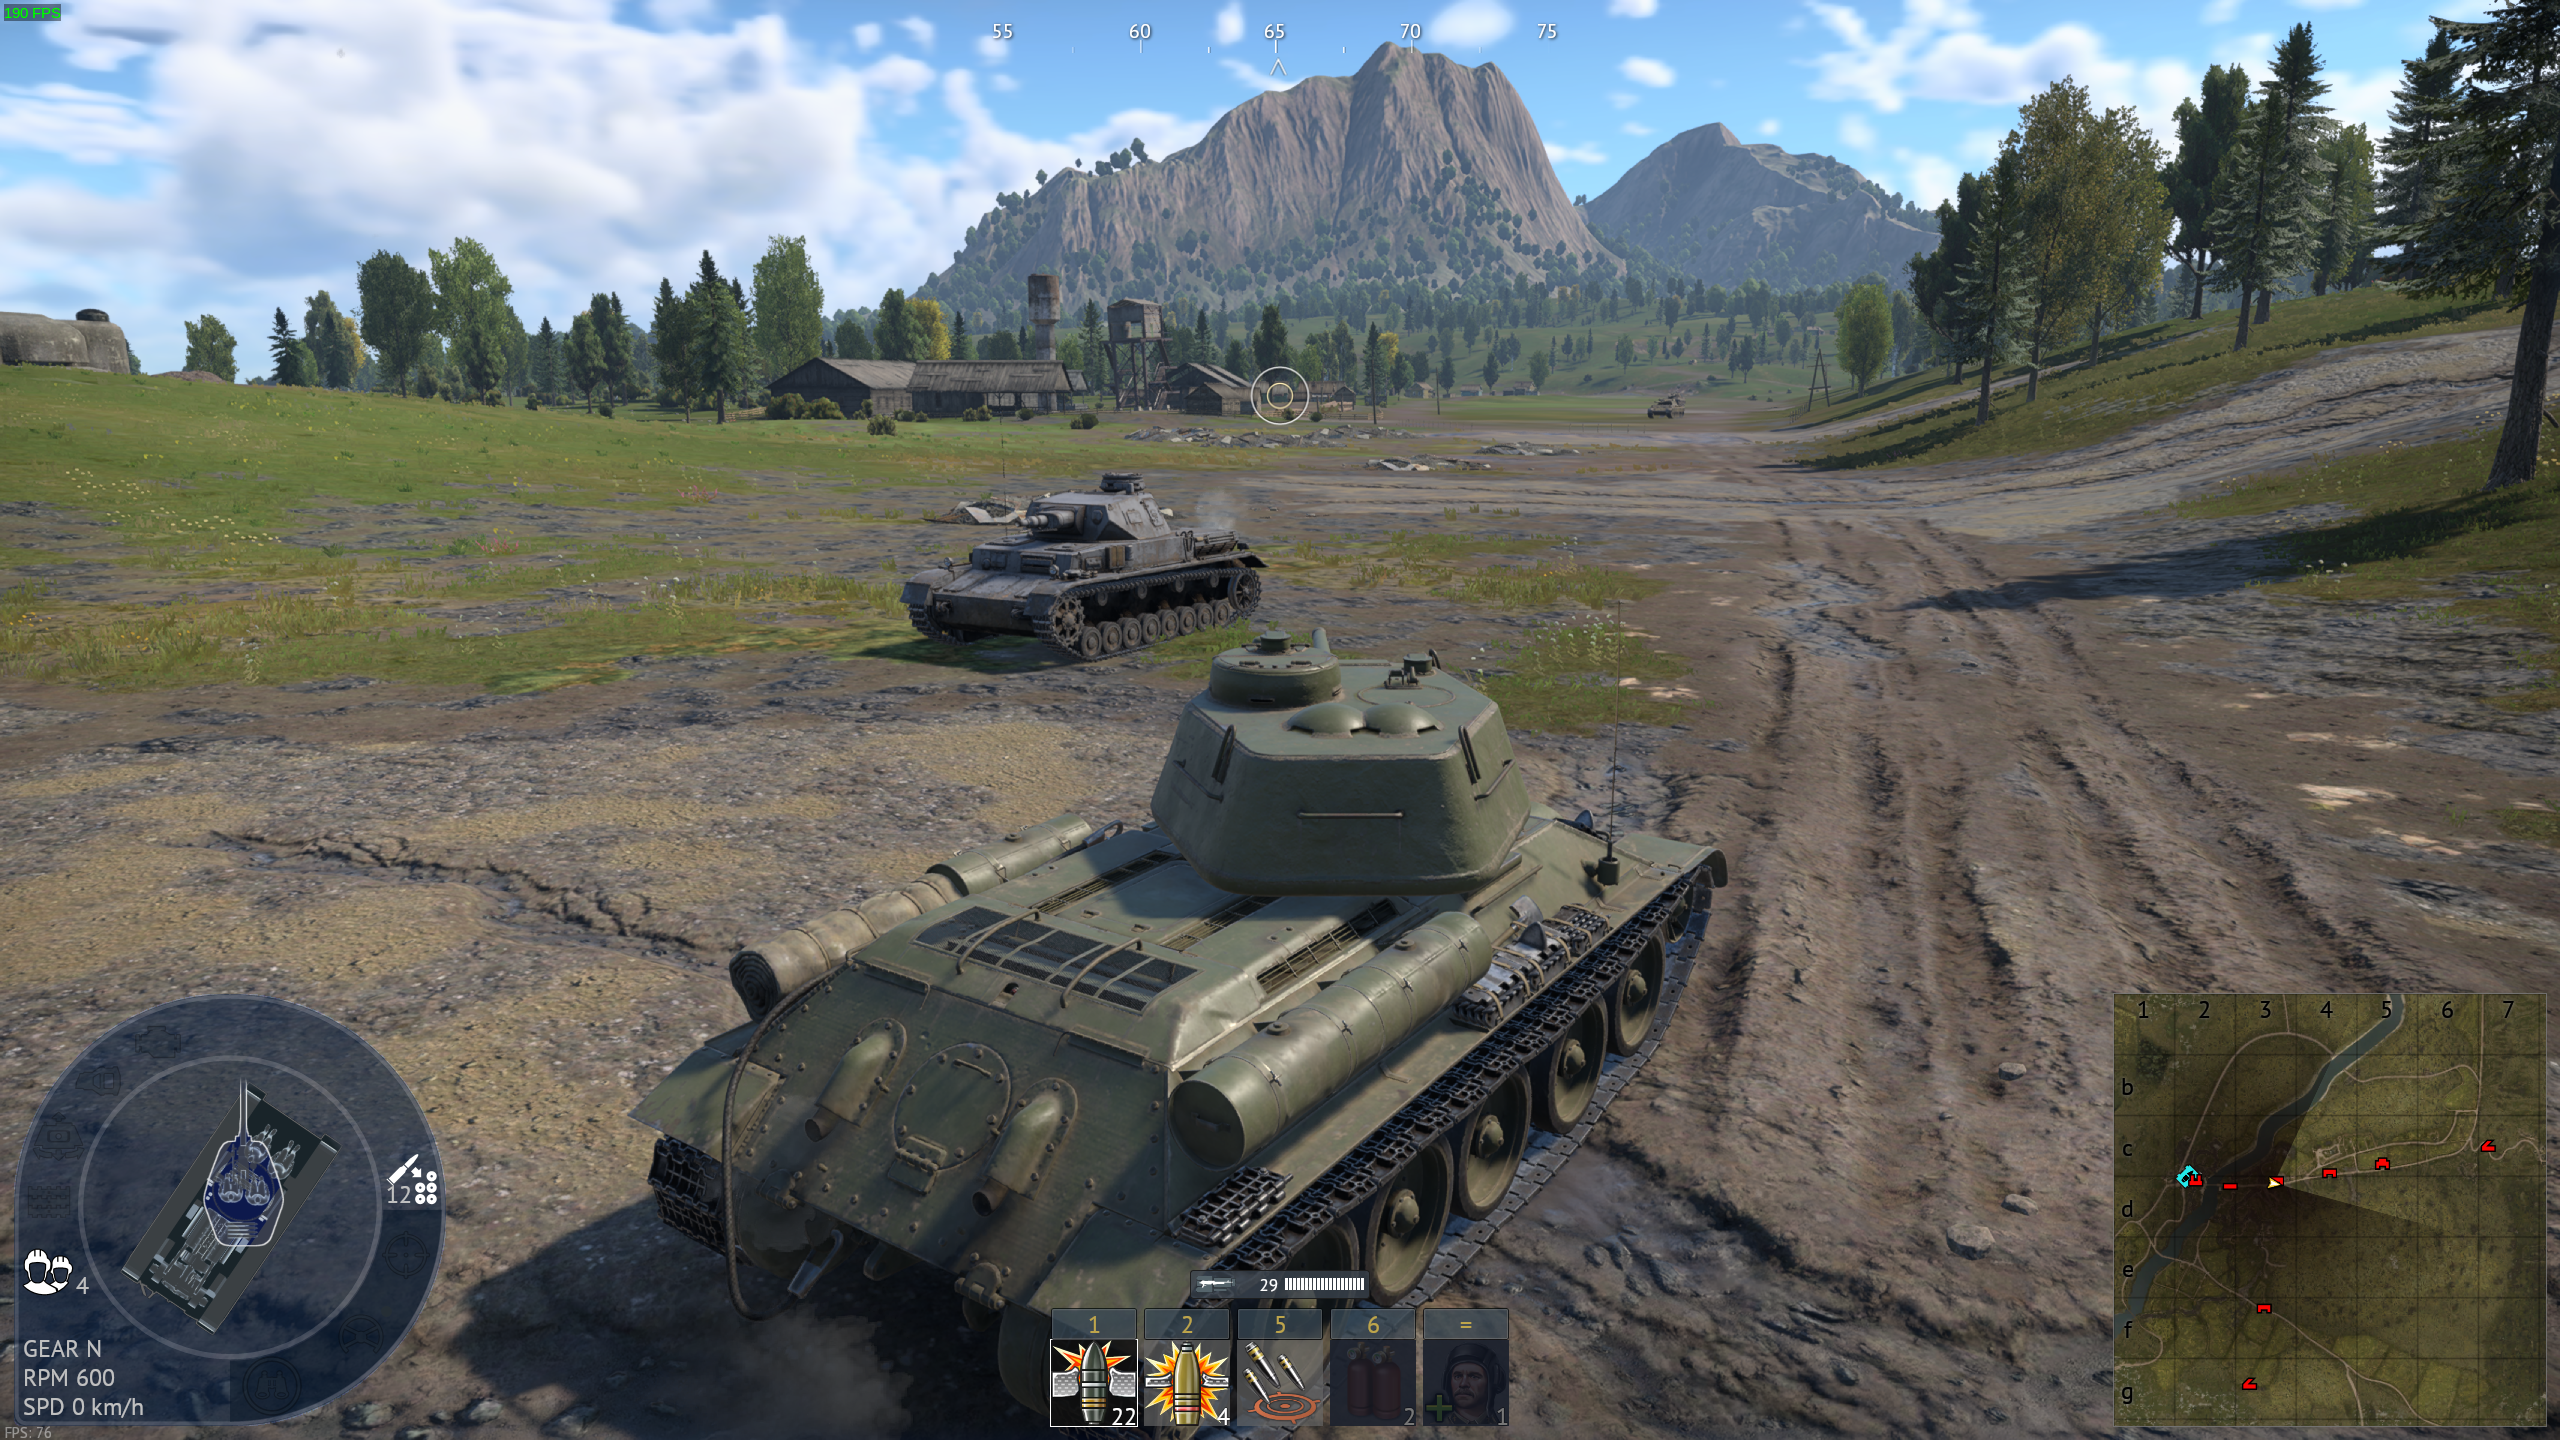
\includegraphics[width=0.9\textwidth]{screenshots/warthundergame.png}
    \caption{Harckocsi modell Blender-ben}
    \label{fig:warthundergame}
\end{figure}


\section{Navmesh}

A Navmesh\cite{navmesh} a mesterséges intelligenciáknál alkalmazott absztrakt adat struktúra, mely segít a komplex környezetekben történő útvonal keresésben. Ez a fogalom már több évtizede ismert a robotika területén, de a 2000-es évek elején népszerűsítették a számítógépes játékok.

Egy két-dimenziós konvex poligonokból\footnote{sokszögekből} álló háló adja meg az ügynök\footnote{Eredeti nevén \emph{agent}} által bejárható területet, melyen belül szabadon mozoghat. Egy poligonon belül egy egyenes vonallal lehet áthaladni, míg két poligon között gráfkereső algoritmusok használatával, mint például az A\* algoritmus, lehet útvonalat találni.

Egy Navmesh-t, bár lehet kézzel készíteni, nagyon hosszadalmas folyamat lenne, ezért általában egy pályán levő statikus geometriában található magasság különbségek alapján van legenerálva.

A szakdolgozatom során tervezem ennek használatát a gépi ellenségek irányításához.

\section{Ray cast}

A ray cast\cite{raycast}\footnote{Sugár követés} egy több évtizede kifejlesztett módszer a 3 dimenziós számítógépes grafikák megjelenítésére 2 dimenziós képernyőkön. Ray cast segítségével el lehet dönteni, hogy adott nézőpontból melyik tárgy van előrébb.

Működése egy pontból kilőtt adott irányba haladó sugárral történik, mely visszaadja az első eltalált pontot, ezzel megállapítva, hogy az adott ponthoz képest mi található a legközelebb egy adott irányban.

Unity-ban ez egy beépített funkció és megadható a sugarak maximális távolsága, valamint a rétegeket.

\section{Quaternion}

\chapter{Felhasznált technológiák}

\section{Unity}

A fejlesztésem alapjának a Unity-t választottam népszerűsége és sokoldalúsága miatt. Rengeteg eszközt ad a fejlesztő kezébe, így szinte bármilyen típusú projektet lehet vele készíteni, akár a játékfejlesztésen túl is.

\subsection{A Unity-ről általánosan}

A Unity játékmotor először 2005-ben jelent meg, amióta folyamatos továbbfejlesztés átváltoztatta teljesen. 2D és 3D játékok feljlesztésére szolgál több platformon is, emellett interaktív szimulációkra használható és virtuális valóságra való fejlesztésre is van támogatása.

Adott bevételig ingyenes lincesszel rendelkezik emiatt az indie és újonc játékfejlesztők körében nagyon elterjedt és tág közösségre tett szert. Emiatt sokféle oktatóvideó található, és rengeteg közösség által készített játék tartozékot (pl. hangok, modellek) lehet letölteni vagy megvásárolni.

\subsection{Gameobject-ek}

Egyik alapeleme a Unity-nek a GameObjectek, melyeknek rengeteg féle felhasználási módjuk van. Bármilyen karakter, pálya vagy tárgy egy GameObject egy jeleneten belül. Alapból nincsen konkrét funkciójuk, de komponenseket lehet hozzájuk csatolni, melyek meghatározás a működésüket. Ezért a GameObjecteket tekinthetjük úgy, mint egy tárolóegység.

\subsection{Komponensek}

\label{sec:components}

A komponensek felelnek a GameObject-ek viselkedéséért, rengeteg különféle funkcionalitást nyújtanak. Alapból rengetek komponens van beépítve a Unity-be, de a szkriptelési funkcionalitással saját komponensekkel lehet ezt a tárat tovább bővíteni. A leggyakrabban használt beépített komponensek:
\begin{itemize}
 \item Transform (Ezt minden GameObject tartalmazza)
 \item Mesh renderer
 \item Collider
 \item Rigidbody
 \item Szkriptek
\end{itemize}

A \emph{Transform} adja meg a pozícióját, méretezését és forgatását az adott objektumnak. A \emph{Mesh renderer} felel a modellek megjelenítésért. A \emph{Collider} az ütközések kezelését szolgálja, több formában is létezik, mint például doboz és kapszula alakú. A \emph{RigidBody} felel a fizikáért. Ezeken kívül még rengeteg beépített komponens létezik.

\subsection{Szkriptelés}

A szkriptek egyféle komponens a GameObjectnek. A játék logikájának és interakcióinak megírására szolgálnak. A szkriptek főként C\# nyelven készülnek, és az egyes játékobjektumok viselkedését, mozgását, valamint a játékbeli eseményeket szabályozzák.


A Monobehavior-ből nevű osztályból öröklődik a legtöbb szkript, mely többféle beépíttet életciklus tesz elérhetővé:

\begin{itemize}
    \item \emph{Start}
    \item \emph{Update}
    \item \emph{FixedUpdate}
    \item \emph{OnCollisionEnter} / \emph{OnTriggerEnter}
\end{itemize}

A \emph{Start} metódus egyszer fut le a szkript indításakor, amikor az adott objektum betöltődik, és az objektum engedélyezve van. Általában inicializálási feladatokhoz van alkalmazva, például változók értékeinek beállítását hajtja végre.

Az \emph{Update} metódus minden képkockánál lefut, így ide kerülnek azok a kódok, amelyeknek folyamatosan, valós időben kell futniuk, például a mesterség intelligenciák irányítása vagy a kezelőfelületen levő folyamatosan frissülő részek.

A \emph{FixedUpdate}, az \emph{Update}-hez hasonlóan, folyamatosan fut, viszont minden fizikai képkockán fut le, a megjelenített képkockáktől függetlenül. Ide a fizikai számítások kerülnek, mivel megadott időközönként fut újra.

Az \emph{OnCollisionEnter} akkor fut le amikor két tárgy amelyek van \emph{Collider} komponense összeütközik. Ütközések vagy fizika lövedékek kezelésére alkalmas.


\section{Blender}

A modellezéshez Blender-t választottam, mely egy ingyenes és nyílt forráskódú 3D modellező és animációs program. A Blender egy nagyon széles körben használt és alkalmazott program a 3D grafika világában, és ingyenessége miatt könnyen kipróbálható és használható.

\begin{figure}[H]
    \centering
    \includegraphics[width=0.9\textwidth]{screenshots/blender.png}
    \caption{Harckocsi modell Blender-ben}
    \label{fig:blender}
\end{figure}

A Blender újabb verzióiban rengeteg eszközzel rendelkezik, mely egyszerűsíti a modellezést és annak tanulását. Emellett tág felhasználói közössége miatt rengeteg segítség található internetes fórumokon, illetve rengeteg tanító videó is áll rendelkezésre, melyek nagyrészben segítettek e programnak a használatában.

\chapter{A játék bemutatása}

\section{A játékmenet}

\subsection{Menü}

A játékot elindításakor a főmenübe kerülünk, ahol 3 gomb fogad, a játékmenet elindítása, beállítások és a kilépés.

A játékmenet elindítására kattintva megjelenik a harckocsi kiválasztására szolgáló menü. Ebben menüben a felső részen a gombok segítségével választhatóak a harckocsi részei, és a gombok között található azoknak a megnevezése. A képernyő közepén látható a jelenleg kiválasztott harckocsi előnézete, mely minden alkatrész váltás során változik. A jobb alsó sarokban található a játék indító gomb, mely indítja a játékmenetet és a bal alsó sarokban a főmenübe visszalépő gomb.


\begin{figure}[H]
    \centering
    \includegraphics[width=0.7\textwidth]{screenshots/selectionmenu.png}
    \caption{Harckocsi választási menü}
    \label{fig:selectionmenu}
\end{figure}

A beállításoknál 3 csúszka található, melyek mellett a jelenlegi értékük található. Ezek szolgálnak a játékbeli érzékenység és a hangerő beállítására.

\begin{figure}[H]
    \centering
    \includegraphics[width=0.7\textwidth]{screenshots/settings.png}
    \caption{Beállítási menü}
    \label{fig:settings}
\end{figure}

\subsection{Csata}

A harckocsi kiválasztása után elindul a csata, ahol egy sziklás pályán jelenik meg a játékos kiválasztott harckocsi, és egy csoport ellenséges harckocsit, melyek egy útvonalat követnek célpontjukig. A játékos célja, hogy az ellenfeleket megsemmisítse mielőtt az ellefnelek a célpontjukhoz érnek. Ha bármelyik ellenfél eléri a célpontot vagy a játékos harckocsija megsemmisül akkor a játékos veszít.

\section{A megvalósítás}

\subsection{A harckocsi}

A \emph{Tank} komponens sok dologért felel. Legfőként a különböző részek létrehozásáért, statisztikáiknak az összekombinálásáért és az életerő-t is kezeli.

\lstinputlisting[caption=A harckocsi létrehozása,label=tankspawn]{./codesnippets/tankspawn.cs}

A \emph{CreateTank} metódus először a gyökér objektumot hozza létre, melyhez hozzáadja a \emph{Tank, Rigidbody} és \emph{BoxCollider} komponenseket. Ezt követően a harckocsi alkatrészeit létrehozza gyerek objektumokként, melyek a többi alkatrész által megadott pozíciókba kerülnek.

Ez a komponens egyéni tapadási fizikáért is felel, mely gyorsabb sebességnél történő fordulásnál nagy mértékben csökkenti a harckocsi sebességét és a fordulás irányába viszi a tankot. Ennek hiányában forduláskor nem lenne tapadás és oldalirányban tudna csúszni. A \emph{SidewaysFriction} a \emph{FixedUpdate}-ben fut le akkor, amikor a harckocsi legalább egyik lánctalpa a földön van.

\lstinputlisting[caption=Tapadási kód,label=tracion]{./codesnippets/traction.cs}

A kód az oldalirányú mozgási sebesség alapján, mely a mozgási irány vektor és az oldal irányi vektor szorzatából kap meg, csökkenti a sebességet a \emph{sidewaysFrictionFactor} alapján. Az értéket tesztelés és érzés alapján állítottam be.

A harckocsi 3 részre van felosztva:
\begin{itemize}
    \item Páncéltest
    \item Lövegtorony
    \item Ágyú
\end{itemize}

Ezentúl, ha a harckocsi élete 0 vagy annál kisebb értékre csökken le, akkor megsemmisültnek számít, mely könnyen észrevehető abból, hogy a lövegtorony lerepül ennek esetén.


\subsubsection{Páncélzati rendszer}
Minden harckocsi modellje fel van osztva több kis darabra, melynek van a beépített \emph{Collider} komponense és a saját páncél komponense. Ezzel a módszerrel pontosan meg lehet adni hogy mely részen mekkora védelme van és mekkora sebzési szorzót kap. Például az ágyúnak és a lánctalpnak kisebb szorzója van, mivel könnyebben átüthető részeknek számítanak, miközben a harckocsi középpontja nem kap sebzést.

\subsubsection{Páncéltest}

Ez a rész adja meg az egész harckocsi teljes sebességét, gyorsulását, a motor hangját és az életerejének a nagy részét. Valamint hozzá tartoznak a lánctalpak is, melyek ellenőrzik, hogy a harckocsi a földön van-e egy adott pillanatban egy rövid sugár segítségével, mely megnézi hogy a terep-be ütközött-e be.  Általánosan ez rendelkezik a legtöbb páncél elemmel is. Valamint a test adja meg a lövegtorony elhelyezkedését. Az ötletet az alábbi projekt alapján kaptam.

\subsubsection{Lövegtorony}

A lövegtorony forgatását a játékos nézőpontjából kilőtt sugár segítségével implementáltam, mely visszaad egy koordinátát, és miután a lövegtorony ezt megkapja, elkezd fordulni megadott sebességgel annak irányába. Emellett a lövegtorony adja meg a belső kamera pozícióját, az ágyú elhelyezkedését is.

\lstinputlisting[caption=Lövegtorony forgatása,label=turretrotation]{./codesnippets/turretrotation.cs}

A \emph{RotateTowards} metódus először megkap egy vektort a célpont pozíciója és a torony pozíciójából, amiből kiszámítja a kívánt irányt. Ezután megkapja \emph{Quaternion}-ban a forgási irányt és végül elkezdi forgatni a tornyot másodpercenként \emph{stats.RotationSpeed} fokkal. Alapul az alábbi kódrészletet\cite{rotation} vettem.

\subsubsection{Ágyú}

Az ágyú emelése hasonlóan működik a toronyhoz forgatásához képest. Viszont megadott a maximum magassági és depressziószögük, melyeken nem mehet túl a függőleges fordulása.

\lstinputlisting[caption=Lövegtorony irányítása,label=barrelelevation]{./codesnippets/barrelelevation.cs}

A kódban sincs túl nagy eltérés a torony forgatásához képest. Viszont itt a 2. sorban a Pitarorasz-tétel\cite{pitagorasz} alkalmazásával a távolgásot megkapom, utána annak segítségével kapom meg a kívánt szöget. Itt figyelembe kellet venni az is, ha a harckocsi emelkedőn van-e. A 7. sorban adom meg a forgási limitet.


\subsubsection{Játékos nézőpontja}

A játékos nézőpontja 2 darab kamerával van megoldva, külső és belső nézetes, melyeknek az érzékenységét külön-külön lehet beállítani. Az egérgörgővel lehet csökkenteni a  kamera látószögét, segíthet nagyobb távolságon történő célzásban.

\subsection{Pálya}

\subsubsection{Kialakítása}

A pálya kialakításához a Unity terepszerkeszőjét használtam, mely ecsetszerű eszközöket segítségével a terepen magasabb és mélyebb részeket lehetett rajzolni. Így egy hegyes-dombos pályát készítettem egy kivájt útvonallal.
\subsubsection{Textúrázás}

A textúrázáshoz szintúgy a terepszerkesztő eszközöket használtam, mellyel az útvonalat egy ecsettel lehetett festeni. A textúrákat a \emph{Poly Haven}\cite{polyhaven} oldalról töltöttem le.

\begin{figure}[H]
    \centering
    \includegraphics[width=0.8\textwidth]{screenshots/mapineditor.png}
    \caption{A Unity szerkesztőjében a pálya}
    \label{fig:mapineditor}
\end{figure}

\subsection{Menü}

\subsubsection{Harckocsi kiválasztása}

A harckocsi részeit a Unity-ba beépített \emph{ScriptableObject}-ek segítségével tudtam eltárolni és ezekből újra elérni a harckocsi kiválasztásakor.

\begin{figure}[H]
    \centering
    \includegraphics[width=0.5\textwidth]{screenshots/scriptableobject.png}
    \caption{\emph{ScriptableObject} kezelőfelülete}
    \label{fig:scriptableobject}
\end{figure}


\subsubsection{Beállítások}

A beállításokban az érzékenységet és a hangerőt lehet állítani, melyekre csúszkák szolgálnak. Ezeket az értékeket egy statikus osztályban tárolom el.


\subsubsection{Szünet menü}

Egy egyszerűbb szünet menü van a játékban, mellyel újralehet indítani a játékmenetet vagy visszamenni a fő menübe. Ilyenkor a játékmenet teljesen megáll illetve a kurzor újra látható és mozgathatóvá válik.

\subsection{Irányítási rendszer}

A bevitelhez a Unity új beviteli rendszerét használtam segítségül, melynek használatával egyszerűen lehetett újabb beviteli billentyűket hozzáadni, valamint azokat csoportosítani és együttesen ki vagy bekapcsolni.

\subsubsection{Célzás}

A célzást az egér mozgásának olvasása teszi lehetővé. A játékmenet közben a kurzor viszont nem látható és a játékablak közepére van lezárva, amíg a játékos fel nem hozza a szünet menüt vagy a játékmenetnek vége nem lesz.

\subsection{Lövedékek}

A lövedékek fizikai objektumként működnek, megadott sebességük és súlyuk van, viszont gravitáció nincs rájuk hatással.

Három féle lövedék van beimplementálva jelenleg a játékba:
\begin{itemize}
    \item páncéltörő
    \item robbanótöltetes pácéltörő
    \item robbanótöltetes lövedék
\end{itemize}

Mindhárom típus egy absztrakt \emph{Bullet} osztályból öröklődik, így a \emph{Start} és az \emph{OnCollisionEnter} metódusaik közösek, valamint implementálniuk kell a \emph{GetMaxPenetration, CalculateDMG} és\emph{CalculatePenetration}.

\lstinputlisting[caption=Absztrakt \emph{Bullet} osztály metódusai,label=bullet]{./codesnippets/bullet.cs}

A \emph{Start} metódusban beállítja a kezdeti pozíciót, az átütés értékét, a sebességet és a méretét a lövedéknek. Az alap méret 100mm-es átmérőre van modellezve, ezért az adott lövedék kaliberével beszorozva megkapjuk az új, pontos méretet.

Az \emph{OnCollisionEnter} ütközéskor fut le, először megnézi hogy ütközött-e páncéllal már, ha igen akkor nem fog sebezi többet. Más esetben megnézi hogy páncéllal ütközik-e és kiszámítja a megtett távolságot a kezdeti pozíciótól. Ha páncélnak számít az eltalált objektum, akkor kiszámítja hogy mennyi átütés maradt meg. Ezután ha maradt még átütési erő, azaz a páncél nem állította meg a lövedéket, akkor sebzi az ellenfelet.


\subsubsection{Páncéltörő lövedék}

A páncél törő lövedék a DeMarre formula alapján lett modellezve. Ez adja meg a súly, átmérő és sebesség alapján a maximális átütési erejét egy adott lövedéknek.

%DeMarr Formula
\begin{equation}
 P_r \times \left( \frac{V}{V_r}\right)^{1,4283} \times \left( \frac{D}{D_r} \right)^{1,0714}  \times \left(\frac{W}{\varnothing}\right)^{0,7143} \div \left(\frac{W_r}{\varnothing_r}\right)^{0,7143}
 \label{demarre}
\end{equation}


Ezentúl a lövedéknek a megtett távolsága és a találat szöge is figyelembe van véve. Ezek befolyásának a mértékét kettő változóval lehet állítani. A távolságnál az 1-es érték figyelmen kívül hagyja a szorzót, az 1 alatti érték, melyet a legtöbb lövedék használ, nagyobb távolságnál csökkenti az átütés mértékét, míg az 1 feletti érték növeli. A szögteljesítménynél az 0-ás érték nem veszi figyelembe a szög mértékét, az 1-es érték a páncélvastagságnak $\cos$ értékét nézi, mely egyenlő az adott szög alapján figyelembe vett vastagságával és a leggyakrabban használt 1 feletti érték gyengíti nagyobb szög esetén. Ha a távolsági és a szögteljesíményi értékeket 1-re állítjuk akkor egy másfajta lövedék típust lehet elérni. Ezekből a változók beállításával lehet további típusokat beállítani.


\lstinputlisting[caption=Átütés kiszámítása,label=APcalculation]{./codesnippets/APcalculation.cs}

A lövedék sebzését, mely maximális értéke kaliberétől és a sebességétől függ, az átütött páncél értékéhez és a lövedék átütő erejétől függően csökkentjük.

\subsubsection{Robbanótöltetes lövedék}

Az alábbi lövedék egy felülethez érvén egy robbanást olyan módon utánoz hogy a megadott átmérőjű gömbön belül először megnézni az összes objektum között hogy bármyelik páncélnak számít-e, majd a robbanás középpontjától számítva mely páncéllemeznek a legkevesebb a vastagsága és a távolságának a keveréke.

\lstinputlisting[caption=Robbanótöltetes lövedék működése,label=hexplosion]{./codesnippets/heexplosion.cs}

A \emph{GetMaxPenetration} egy sajátos függvényt használ az átütés kiszámítására, itt az értékeket a \emph{War Thunder} lövedékéihez képest hasonlóra szerettem volna megoldani, de azzal nem egyezik meg.

A \emph{CalculatePenetration} a leggyengébb páncél alapján adja vissza a maradandó átütést. Ezt a \emph{GetWeakestArmor} metódus segítségével kapja meg, mely először megnézi az összes \emph{Collder}-el rendelkező objektumot egy adott távolságon belül. Utána \emph{Ray cast}-ok segítség megnézim hogy a robbanás középpontjából látható-e az adott objektum, melyet a pozícióik összehasonlításával ellenőriz, figyelmen kívül hagyva a \emph{CollisionBox} réteget. Ezután megnézi, hogy az adott objektum páncél-e. Ha ténylegesen páncél, akkor megnézi az ellenállását a \emph{GetResistance} fügvénnyel, mely a távolság szerint növeli a páncél védelmének erejét négyzetesen.


\subsubsection{Robbanótöltetes páncéltörő lövedék}

Ez a lövedék hasonlóan működik a sima páncéltörő lövedékhez képest, az átütő ereje ugyanazon a módon van kiszámítva. A különbség a sebzés kiszámításában van, de csak akkor lép életbe, ha a lövedék egy adott vastagsága páncélt átütött, miután a robbanótöltet mértékétől függően sebez.



\subsection{Kezelőfelület}

\subsubsection{Életerő sáv}

Két féle életerő sáv létezik a projektben. Az első típusú a kezelőfelületen fixen található a bal alsó sarokban, mely számokkal kijelzi a teljes és a jelenlegi életerőt, illetve hiányzó életerő mértéke szerint kevesebb része lesz kitöltve a sávnak. A másik típus az ellenfelek felett megtalálható, és a 3D térben helyezkednek el.
\begin{figure}[H]
    \centering
    \includegraphics[width=0.5\textwidth]{screenshots/hpbar.png}
    \caption{Életerő sávok}
    \label{fig:healthbar}
\end{figure}


\subsubsection{Célkereszt}

A célkereszt 2 részből áll. A kör alakú irányzék a képernyő közepét és a kívánt célpontot jelzi, emellett lövés után pirossá változik, jelezve az újratöltés menetét. A második, kereszt alakú, pedig azt jelzi, hogy a cső jelenleg milyen irányba néz.

\begin{figure}[H]
    \centering
    \includegraphics[width=0.5\textwidth]{screenshots/crosshair.png}
    \caption{Célkeresztek}
    \label{fig:crosshair}
\end{figure}

\subsection{Hangok}

A játékban csak 2 féle hang van jelenleg implementálva: a motor hang és a lövés hang.
A motor hangja folyamatosan ismétlődve játszódik le, és a hangmagassága a sebesség szerint növekszik vagy csökken. A lövési hang természetesen csak lövés esetén hallható. A hangokat az alábbi oldalról\cite{freesound} töltöttem le.

\subsection{Ellenfelek}

\subsubsection{Navmesh}

Az ellenfelek útkeresését a Unity-nak a beépített Navmesh rendszere segítségével implementáltam. Bár a Navmesh-be alapból van megadott módszer a mozgásra, de az emberszerű karakterekre van tervezve. Emiatt a sajátos mozgási megoldásra kellett hagyatkozzak. Így ugyanazt a mozgási rendszert használják mint a játékosok.

\subsubsection{Ellenőrző pontok}

Az ellenfeleknek van egy megadott útvonaluk amit követnek, melyet ellenőrző pontok segítségével oldottam meg. Amikor
az adott ellenfél belép egy adott ellenőrző pont érzékelőpont

\lstinputlisting[caption=Ellenőrző pontok váltása,label=checkpoints]{./codesnippets/checkpointsystem.cs}


\subsubsection{Állapotgép}

Állapotgép használatával van megoldva az ellenfelek viselkedésének szétválasztása. Azért választottam állapotgépet ehhez, mert egy tiszta és egyszerűen bővíthető módszert ad különböző viselkedések és állapotok megadására.

\lstinputlisting[caption=Lövegtorony irányítása,label=statemachine]{./codesnippets/statemachine.cs}

\subsubsection{Állapotok}

Kétféle állapot van:
\begin{itemize}
 \item Járőrözés
 \item Támadás
\end{itemize}

\subsubsection{Járőrözés}

A járőrözés az alap állapot, melyben az ellenőrző pontok által megadott útvonalat követi az ellenfél.

\subsubsection{Támadás}

Erre az állapotra akkor vált az az ellenfél, ha az ellenfél előtt elmegyünk és akadály nélkül meglát. Átváltás után amíg a játékos nem kerül akadály mögé, addig az ellenfél a testét és a tornyát forgatja a játékos felé. Miután sikeresen célba vette a játékost az ellenfél lő. Ha a játékos kimegy az ellenfél látószögéből akkor az ellenfél megpróbálja utolérni a játékost. Ha adott időn belül nem látja meg újra a játékost, akkor az ellenfél visszatér járőrözési állapotba.

\lstinputlisting[caption=Állapotgép,label=checkplayervisible]{./codesnippets/checkplayervisible.cs}

\section{További tervek}

A projektnek az alapját és a fő funkcióit sikerült eddigiekben kifejleszenem. Ezentúl szeretném ezt továbbfejleszteni, és kiegészíteni.

\subsubsection{Tartalom}

A projektem alapja miatt jelenleg készen áll több tartalom fogadására, mely alatt főleg nagyobb harckocsi alkatrésztár és újabb pályák értendőek.

\subsubsection{Funkciók}

Funkciók közül több ötletem is támadt a fejlesztés közben amikkel szeretném kiegészíteni a továbbiakban. Amit a legfontosabbnak tartok az a billentyűk megváltoztatásának lehetősége lenne, a testreszabhatóság érdekében, és a kontrolleres bevitel támogatása.
Emellett további tervekben többféle ellenfél viselkedést és játékmódot implementálni, valamint animációkat és esetleges fizikát a lánctalpakhoz.



\chapter{Tesztelés}

Teszteléshez manuális tesztelést alkalmaztam.


\chapter*{Összegzés}
\addcontentsline{toc}{chapter}{Összegzés}




\begin{thebibliography}{55}

    \bibitem{warthunder}
    \textsc{Gaijin Entertainment } \emph{War Thunder Wiki} \\
    \url{https://wiki.warthunder.com/}

    \bibitem{navmesh}
    \textsc{Wikipedia} \emph{Navigation mesh} \\
    \url{https://en.wikipedia.org/wiki/Navigation_mesh}

    \bibitem{raycast}
    \textsc{Wikipedia} \emph{Ray casting} \\
    \url{https://en.wikipedia.org/wiki/Ray_casting}

    \bibitem{unity}
    \textsc{Unity} \emph{Unity Documentation} \\
    \url{https://docs.unity.com/}

    \bibitem{rotation}
    \textsc{Unity Forums} \emph{Rotate towards target position (mouse) at a limited speed} \\
    \url{https://discussions.unity.com/t/rotating-slowly-toward-a-target-while-also-moving-toward-that-target/886726}

    \bibitem{pitagorasz}
    \url{https://hu.wikipedia.org/wiki/Pitagorasz-t\%C3\%A9tel}

    \bibitem{demarre}
    \textsc{The Tank Archives} \emph{Penetration Equations} \\
    \url{https://www.tankarchives.ca/2014/10/penetration-equations.html}

    \bibitem{freesound}
    \textsc{Freesound} \emph{Freesound} \\
    \url{https://freesound.org/}


    \bibitem{polyhaven}
    \textsc{Poly Haven} \emph{The Public 3D Asset Library} \\
    \url{https://polyhaven.com/}

\end{thebibliography}
\addcontentsline{toc}{chapter}{\bibname}

\end{document}
